\documentclass{article}
\usepackage[utf8]{inputenc}
\usepackage{tikz}
\usepackage{graphicx}
\graphicspath{ {./images/} }

\title{CS132 Quizzes - Memory Systems}
\begin{document}
\begin{center}
    \Huge\textbf{CS132 Quizzes - Memory Systems}\\
    \huge\textit{May 2021}\\
    \medskip
    \Large\textit{Edmund Goodman}
\end{center}




\section{Give four factors that influence the selection of an appropriate memory
technology}

\begin{enumerate}
\item
  Cost of production
\item
  Access speed
\item
  Frequency of access
\item
  Capacity
\end{enumerate}


\section{Explain the ``designer's dilemma'' for memory systems}

The designers dilemma is the trade-off in designing memory which is fast, high
capacity, and cheap to manufacture. It is not possible to design memory which
achieves all of the properties, so the dilemma is how to select which ones to
best fit the use case


\section{Explain, using a diagram, the memory hierarchy}

The memory hierarchy is a way of approaching the designers dilemma to get the
best of each of the properties.

Small amounts of very fast, frequently accessed memory close to the microprocess
(registers and cache) are used to allow the computer to perform operations very
quickly, without having all of the memory of this type, as that would limit
capacity and cost a huge amount.

Further away from the microprocessor, slower, higher capacity and cheaper memory
is used to store data which is less commonly accessed, so high speeds are not
needed.

The diagram below shows a representation of the memory hierarchy:

\begin{figure}
\centering
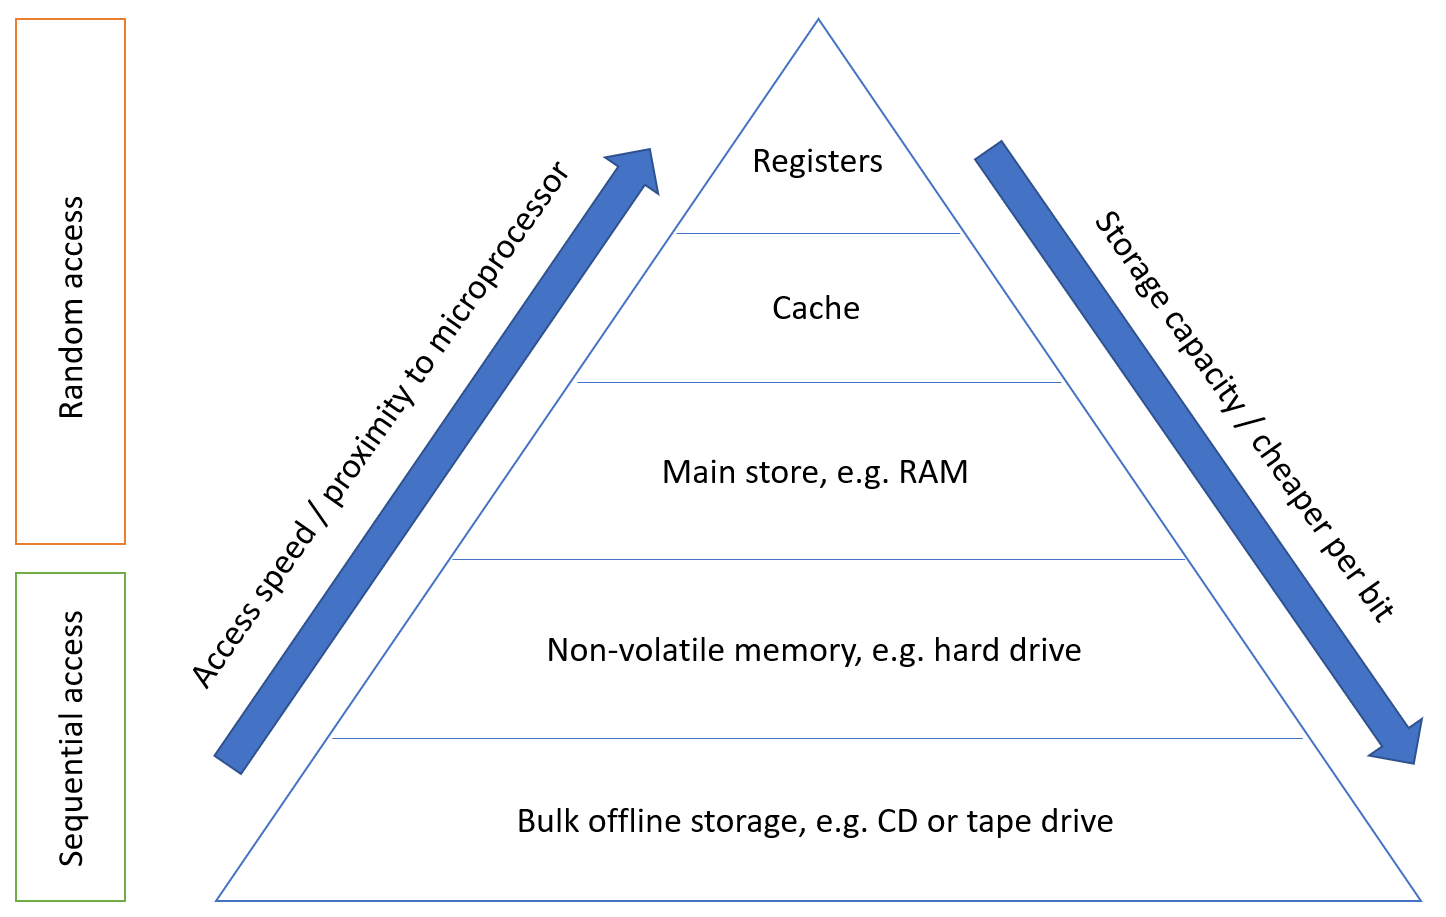
\includegraphics[width=\textwidth]{./memoryHeirarchy.png}
\caption{The memory heirarchy}
\end{figure}


\section{Explain the role of cache memory}

Cache memory is a small amount (typically tens of kilobytes) of memory near the
microprocessor which can be accessed very quickly. Cache memory can be used to
store values in memory which are likely to be retrieved, so the read times are
quicker than out of the main store

In computer systems, the next memory location to be accessed is very likely to
be close to the previous memory location accessed. Cache memory often copies the
memory locations around the last memory location, which means that a significant
amount of the time, the cache already has the memory needed, increasing read
speeds


\section{How can cache memory exploit spatial locality}

Spatial locality is the idea that memory adjacent to the program counter
position is much more likely to be accessed next than other memory in the
computer (estimates say that 90\% is within 2 kilobytes to either side). This
means that the cache can store this memory, allowing faster access then if it
had to look it up in the main store


\section{How can cache memory exploit temporal locality}

Temporal locality is the idea that some memory is more likely to be used in the
future. If an estimate of what this likely memory is can be made, it can be
stored in the cache, allowing faster access then if it had to look it up in the
main store


\section{Explain, using a worked example, how a parity bit can be used to detect
errors. You should state the types of error that your scheme is capable of
detecting and correcting}

A parity bit is an additional bit of information included with data to be sent
used to detect errors that occur in its transmission.

There are two types of parity, odd and even parity. In even parity, the
additional parity bit is used to make the number of the number of ones and the
number of zeroes in a transmission both even. For example, in 8-bit parity, if
the 7-bit message: ``0101001'' is sent, then even-parity would add the parity
but ``1'' to the end to make the message ``''0101001 1'', so the number of zeros
and the number of ones are both even. In odd parity, the same process is
applied, but the digit is added to make both numbers odd.

This error checking scheme can detect when an odd number of bits in the
transmission have been changed (when an even number are changed, it presents as
correct, even though bits have been flipped). This means that whilst it is
robust against single errors, bursts of errors make it only around 50\%
effective.

There is no way to identify where the error occurred, so if an error is
detected, it is corrected by replying to the sender that a re-transmission is
needed


\section{Explain, using a worked example, how error correcting codes can use
bit- and column-parity to detect and correct errors. You should state the types
of error that your scheme is capable of detecting and correcting}

Bit and column parity extends using single parity bits, by not only having a
parity bit at the end of each ``word'', e.g. a byte with 7 bits of message and
one of parity, but also sending a parity ``word'' after a group of words in the
same way of a parity bit after a group of message bits.

For example, in even parity:

\begin{quote}
0101010 1 0110011 0 0111000 1 0110100 1 0101000 0 0111100 0 0000011 0
\end{quote}

The parity word at the end is a parity bit of the column - for example, the
first column is 0000000, so the parity bit would be another 0. In this example,
the parity word is 0000010, with each being the parity bit of the column.

All burst errors, up to 14 bits can be identified using this schema, and they
can be corrected by looking up the failed parity bit by which row and which
column had incorrect bits, and flipping them











\end{document}
